\documentclass{standalone}

\usepackage[T1]{fontenc}
\usepackage[utf8]{inputenc}
\usepackage{amsmath}
\usepackage{tikz}
% ACM style
%\usepackage{newtxmath}
%\usepackage{libertine}
%\usepackage{inconsolata}
% IEEEtrans style
\usepackage{mathptmx}
\usepackage{color}

\usetikzlibrary{fit}
\usetikzlibrary{positioning}

\definecolor{Paired-1}{RGB}{31,120,180}
\definecolor{Paired-2}{RGB}{166,206,227}
\definecolor{Paired-3}{RGB}{51,160,44}
\definecolor{Paired-4}{RGB}{178,223,138}
\definecolor{Paired-5}{RGB}{227,26,28}
\definecolor{Paired-6}{RGB}{251,154,153}
\definecolor{Paired-7}{RGB}{255,127,0}
\definecolor{Paired-8}{RGB}{253,191,111}
\definecolor{Paired-9}{RGB}{106,61,154}
\definecolor{Paired-10}{RGB}{202,178,214}
\definecolor{Paired-11}{RGB}{177,89,40}
\definecolor{Paired-12}{RGB}{255,255,153}

\begin{document}
  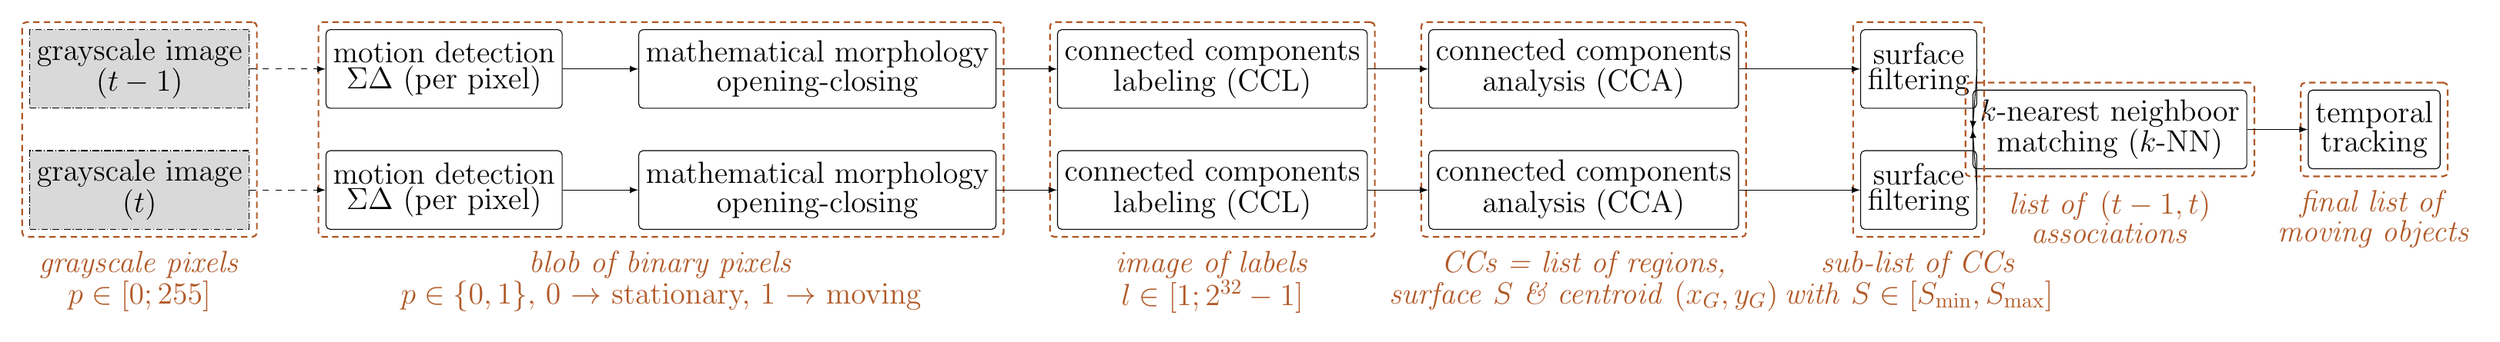
\begin{tikzpicture}%[scale=\tikzscale]
    \tikzset{ tsk/.style={draw=black, rounded corners=2pt, text=black, minimum height=1.3cm, minimum width=1cm} }
    \tikzset{ img/.style={draw=black, densely dashdotted, rounded corners=0pt, text=black, minimum height=1.3cm, minimum width=1.5cm, fill=black!15} }
    \tikzset{ com/.style={draw=Paired-11, densely dashed, rounded corners=2pt, thick} }

    \node[img,                      align=center] (t1)  at (0.0, 1.0)  {{\Large {grayscale image}}\\{\Large $(t-1)$}};
    \node[tsk, right=1.25cm of t1,  align=center] (t2)                 {{\Large {motion detection}}\\{\Large {$\Sigma\Delta$ (per pixel)}}};
    \node[tsk, right=1.25cm of t2,  align=center] (t3)                 {{\Large {mathematical morphology}}\\{\Large {opening-closing}}};
    \node[tsk, right=1.00cm of t3,  align=center] (t4)                 {{\Large {connected components}}\\{\Large {labeling (CCL)}}};
    \node[tsk, right=1.00cm of t4,  align=center] (t5)                 {{\Large {connected components}}\\{\Large {analysis (CCA)}}};
    \node[tsk, right=2.00cm of t5,  align=center] (t6)                 {{\Large {surface}}\\{\Large {filtering}}};

    \node[img,                      align=center] (t1b) at (0.0, -1.0) {{\Large {grayscale image}}\\{\Large $(t)$}};
    \node[tsk, right=1.25cm of t1b, align=center] (t2b)                {{\Large {motion detection}}\\{\Large {$\Sigma\Delta$ (per pixel)}}};
    \node[tsk, right=1.25cm of t2b, align=center] (t3b)                {{\Large {mathematical morphology}}\\{\Large {opening-closing}}};
    \node[tsk, right=1.00cm of t3b, align=center] (t4b)                {{\Large {connected components}}\\{\Large {labeling (CCL)}}};
    \node[tsk, right=1.00cm of t4b, align=center] (t5b)                {{\Large {connected components}}\\{\Large {analysis (CCA)}}};
    \node[tsk, right=2.00cm of t5b, align=center] (t6b)                {{\Large {surface}}\\{\Large {filtering}}};
    \node[tsk,                      align=center] (t7)  at (32.5, 0.0) {{\Large {$k$-nearest neighboor}}\\{\Large {matching ($k$-NN)}}};
    \node[tsk, right=1.00cm of t7,  align=center] (t8)                 {{\Large {temporal}}\\{\Large {tracking}}};

    \node[com, label={[Paired-11, yshift=-0.1cm, align=center]below:{\Large \textit{grayscale pixels}}\\ {\Large $p \in [0;255]$}},  fit=(t1) (t1b)] (o1) {};
    \node[com, label={[Paired-11, yshift=-0.1cm, align=center]below:{\Large \textit{blob of binary pixels}}\\ {\Large $p \in \{0,1\}$, 0 $\rightarrow$ stationary, 1 $\rightarrow$ moving}},  fit=(t2) (t2b) (t3) (t3b) ] (o2) {};
    \node[com, label={[Paired-11, yshift=-0.1cm, align=center]below:{\Large \textit{image of labels}}\\ {\Large $l \in [1;2^{32}-1]$}}, fit=(t4) (t4b) ] (o3) {};
    \node[com, label={[Paired-11, yshift=-0.1cm, align=center]below:{\Large \textit{CCs = list of regions,}}\\ {\Large \textit{surface} $S$ \textit{\& centroid} $(x_G,y_G)$}}, fit=(t5) (t5b) ] (o4) {};
    \node[com, label={[Paired-11, yshift=-0.1cm, align=center]below:{\Large \textit{sub-list of CCs}}\\ {\Large \textit{with} $S \in [S_\text{min}, S_\text{max}] $}}, fit=(t6) (t6b) ] (o5) {};
    \node[com, label={[Paired-11, yshift=-0.1cm, align=center]below:{\Large \textit{list of} $(t-1,t)$}\\ {\Large \textit{associations}}}, fit=(t7)] (o6) {};
    \node[com, label={[Paired-11, yshift=-0.1cm, align=center]below:{\Large \textit{final list of}}\\ {\Large \textit{moving objects}}}, fit=(t8)] (o7) {};

    \draw[->,>=latex, dashed] (t1.east)  -- (t2.west)  node [midway, above] {};
    \draw[->,>=latex        ] (t2.east)  -- (t3.west)  node [midway, above] {};
    \draw[->,>=latex        ] (t3.east)  -- (t4.west)  node [midway, above] {};
    \draw[->,>=latex        ] (t4.east)  -- (t5.west)  node [midway, above] {};
    \draw[->,>=latex        ] (t5.east)  -- (t6.west)  node [midway, above] {};

    \draw[->,>=latex, dashed] (t1b.east) -- (t2b.west) node [midway, above] {};
    \draw[->,>=latex        ] (t2b.east) -- (t3b.west) node [midway, above] {};
    \draw[->,>=latex        ] (t3b.east) -- (t4b.west) node [midway, above] {};
    \draw[->,>=latex        ] (t4b.east) -- (t5b.west) node [midway, above] {};
    \draw[->,>=latex        ] (t5b.east) -- (t6b.west) node [midway, above] {};

    \draw[->,>=latex        ] (t6.east)  -- (t7.west)  node [midway, above] {};
    \draw[->,>=latex        ] (t6b.east) -- (t7.west)  node [midway, above] {};
    \draw[->,>=latex        ] (t7.east)  -- (t8.west)  node [midway, above] {};
  \end{tikzpicture}
\end{document}